\chapter{Abstract}
\label{ch:Abstract}

With the ever increasing amount of data to be rendered for a single given scene, experimenting with new approaches for handling and structuring that data becomes more and more important. This paper covers the approach to enhance response times and quality using out-of-core techniques. \\

With the help of out-of-core techniques, it is possible to achieve real-time rendering performance on current-generation graphics cards by overcoming limits posed by the graphics cards' internal memory \cite{Crassin:2009:GRS:1507149.1507152}. Thus, this topic is essential for everyone hoping to achieve such performance for scenes that cannot be efficiently rendered using conventional methods. \\

I will discuss different strategies used to load necessary data chunks into working memory taking into account its finiteness using intelligent data streaming. These include visibility culling and virtual texturing. Also, this paper will give an overview of the possibility to use volumetric texture units called ``Voxels'' instead of regular texels and the advantages and challenges that come with it. Lastly, the topic will be further explored using the examples \cite{Crassin:2009:GRS:1507149.1507152} and \cite{van2009id}.

\chapter{Motivation}
\label{ch:Motivation}

Over the course of the last years, the complexity of scenes to be rendered has risen further and further. Nowadays, performance and complexity demands cannot be satisfied by solely utilizing brute force methods and trying to fit all necessary data into the scarce graphics memory. There are a number of specific use cases where another approach is needed. For example, \cite{10.1007/978-3-540-40014-1_3} look for a way to interactively render very large landscapes in the context of virtual reality using commmodity graphics hardware. Further, \cite{Gobbetti:2005:FVM:1073204.1073277} name the fields of 3D scanning, computer-aided design and numerical simulation.

In essence, all of these use cases require a technique able to expand available memory by making use of larger but slower storage. While doing this, the searched technique should also minimize response times which are bound to increase due to longer memory access times. A technique that finds a suitable compromise between memory extension and response times is called an Out-of-Core technique.

\chapter{Basics}
\label{ch:Basics}

This chapter aims to introduce key terminology that will be used in this paper. The chapter gives a basic understanding of the terms ``Texture Mapping'', ``Memory Virtualization'', ``Virtual Texture'' and ``Level of Detail''.

\section{Texture Mapping}

Texture mapping provides a way of adding detail to rendered surfaces without increasing geometric complexity. In its simplest form, it takes a 2-dimensional image called \textit{texture map} and a 3-dimensional model and paints the image onto the model. \textit{Texture coordinates} are used to determine which point on the texture map corresponds to a point on the model.

\begin{figure}[h]
  \begin{center}
    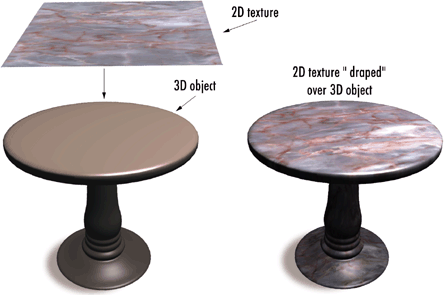
\includegraphics[width=.3\textwidth]{logos/texture_mapping_example.png}
    \hfill
    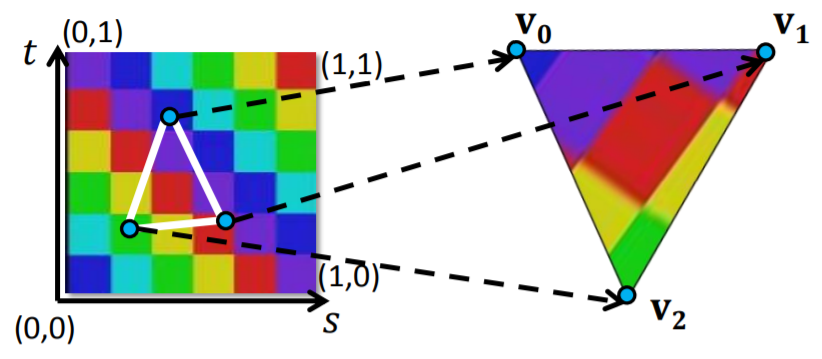
\includegraphics[width=.5\textwidth]{logos/texture_coordinates_example.png}
    \caption{Left: A texture is mapped onto the table model, making it more realistic. Right: 3D points are translated to texture coordintates to determine vertex color. Images from \cite{TextMapExample} and \cite{CompGraphics:2017:04:TexMap}}
  \end{center}
\end{figure}

The first notable paper about texture mapping was published by \cite{catmull1974subdivision} in 1974. After that, texture mapping became particularly popular in video games of the 90's and is now a crucial part of the vast majority of computer-rendered scenes. Because of its usefulness, the concept of texture mapping was extended from affecting the diffuseness to also altering other aspects like specularity, lighting and normals.

\section{Memory Virtualization}

Memory virtualization is the process of abstracting from the physical memory available. The initial motivation for this concept was to enable the uniform usage of heterogeneous storage devices \cite{Euler:VirtualMemoryHistory:2008}. However, it also has more advantages. Firstly, memory fragmentation is reduced, decreasing average memory access times. Secondly, virtual memory can combine (graphics) main memory and slower storage and thus increase the total space available to load data into. Other aspects of memory virtualization are beyond the scope of this paper. The most important aspect of memory virtualization regarding rendering large amounts of data is its ability to extend available memory as this solves one of the issues mentioned in \ref{ch:Motivation}.

The Windows Display Driver Model v2.0 supports graphics memory virtualization under Windows 10 \cite{Microsoft:GPUVirtualMemory:2017}. However, page faults cause rendering to halt until the requested page is loaded. This makes this solution unsuitable on its own as it reduces responsiveness.

\section{Virtual Texture}

A virtual texture is, in general, a texture too large to fit into the physical graphics memory that is available in virtual memory. 

\begin{figure}[h]
  \begin{center}
    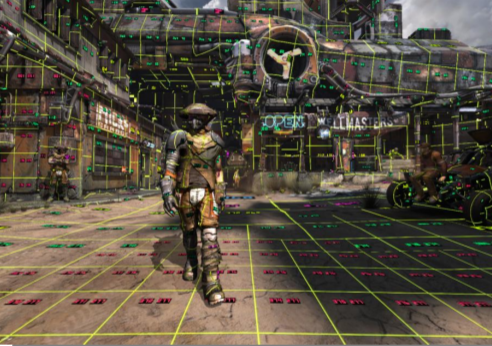
\includegraphics[width=.3\textwidth]{logos/virtual_texture_example.png}
    \caption{Image only shows a tiny portion of the actual virtual texture. Different levels of detail can be seen. Image from \cite{van2009id}}
  \end{center}
\end{figure}

The advantage of a virtual texture over a conventional physical texture is its ability to hold significantly larger amounts of rendering data. For example, id Tech 5 uses virtual textures that consist of approximately 16.3 billion texels \cite{van2009id}. Without special handling, virtual textures face the same responsiveness issues as virtual memory.

\section{Level of Detail}

Level of Detail refers to altering an object's complexity between rendered frames. An example of this technique applied to textures is mip-mapping. 

\begin{figure}[h]
  \begin{center}
    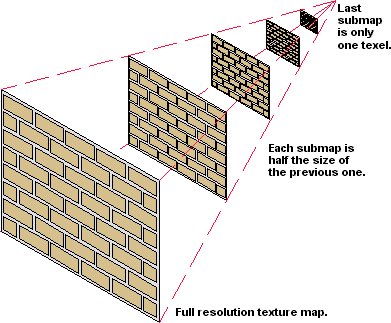
\includegraphics[width=.3\textwidth]{logos/mipmap_example.png}
    \caption{A texture is saved at different resolutions. As the viewer moves closer, resolution is increased and vice versa. Image from \cite{PCMag:DefMipMapping:2017}}
  \end{center}
\end{figure}

Level of Detail addresses the issue of increasing scene complexity as the viewpoint moves away from a limited clip and its environment moves into view. Decreasing the complexity of the objects furthest away from the camera increases rendering performance while not significantly affecting quality \cite{Unity:LevelOfDetail:2017}. Hence, Level of Detail can be used to address the aspect of responsiveness mentioned in \ref{ch:Motivation}.

\chapter{Main Content}
\label{ch:MainContent}

\section{Memory Management}

This section covers ways to utilize slow external memory to be able to store large datasets without losing wanted performance.

Once datasets reach a certain size it simply becomes impossible for them to be held inside the graphics card's main memory. This implies the need for using slower storage devices to reach sufficient capacity. However, simply separating the dataset in question into chunks small enough to be completely loaded into working memory leads to a worst case performance bad enough to prohibit real time performance. In conclusion, \textit{intelligent data streaming} has to be used to ensure having all needed data at hand without significant performance losses \cite{Crassin:2009:GRS:1507149.1507152}. The trade-off to consider here is transferring as little data as possible at a time to minimize processing delays on the one hand and keeping the number of necessary data transfers at a minimum on the other hand. A number of approaches to solve this issue have been developed.

A rather simple solution to extending the available memory is to transfer the idea of virtual pages and physical frames used by operating systems into the given context. 

\begin{figure}[h]
  \begin{center}
    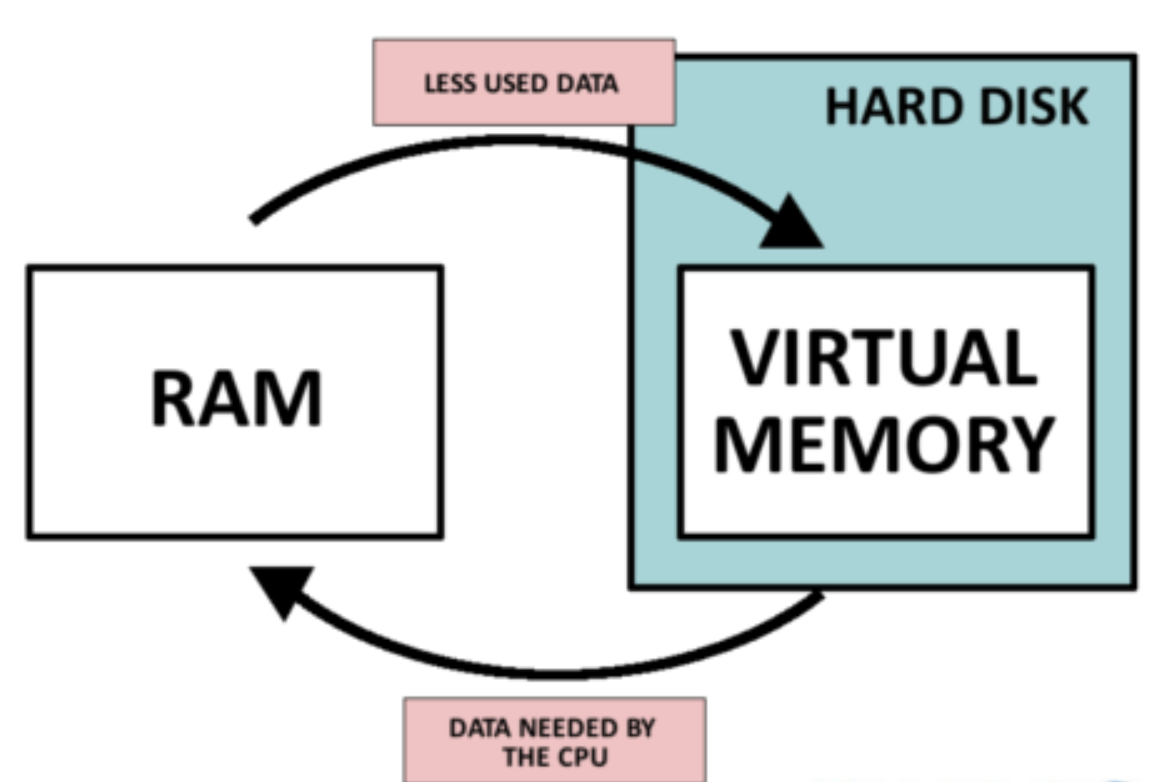
\includegraphics[width=.3\textwidth]{logos/virtual_memory_concept.png}
    \caption{RAM is extended with part of the hard disk. Data is streamed to the RAM on demand, being exchanged for less used data. Image from \cite{TechICT:VirtualMemory}}
  \end{center}
\end{figure}

This introduces a small unit of data chunk that can be loaded into working memory on demand rather quickly. Furthermore, replacement strategies known from the operating system context can also be used, ensuring that often used data is kept in the graphics card memory as much as possible. However, for very large virtual textures even these small chunks lead to physical memory oversubscription. This, in turn, causes page thrashing which results in new frames being processed at a high latency \cite{van2009id}. As most datasets requiring Out-of-Core techniques have comparable texture sizes, this approach is not sufficient.

A more sophisticated approach is to continuously monitor the physical space demand and reduce some portions of information if the graphics card memory capacity is exceeded. For this, both a policy of portioning the data and a strategy for determining which piece of information should be compressed need to be formed. The portioning can be achieved by \textit{tiling}, i.e. cutting the virtual texture into many small tiles of equal size. In general, Level of Detail is used for determining which texture tiles can be swapped and can, for example, be combined with mip-mapping \cite{Crassin:2009:GRS:1507149.1507152}. For instance, as the viewer moves away from the scene more texels move into view and therefore have to be loaded. However, the pixel footprint of the texels that are already loaded becomes smaller. This means that less detail is required and the relevant parts of the texture can be replaced with lower-resolution versions if memory becomes scarce. This solution provides a rendering algorithm that is able to adapt to changing memory demands while limiting performance loss. Details about the storage of textures and update policies will be discussed in the examples.

\section{Voxels}

This section gives a detailed overview of the concept of voxels. It outlines their differences to texels, advantages, challenges and their suitability for out of core processes.

The term \textit{voxel} firstly differs from the texel in that its prefix is taken from the word ``volume'' rather than ``texture''. Thus, it does not stand for a 2-dimensional element of a flat texture but makes up part of a 3-dimensional texture volume. Analogous to a texel often having the shape of a square, a voxel can, but does not have to be cubic.

\begin{figure}[h]
  \begin{center}
    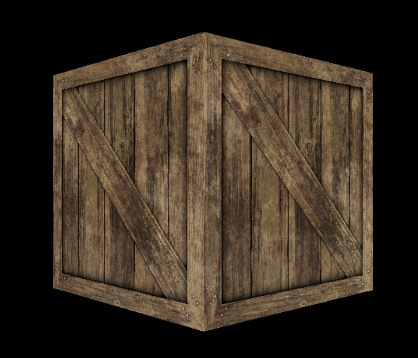
\includegraphics[width=.4\textwidth]{logos/texel_textured_cube.png}
    \hfill
    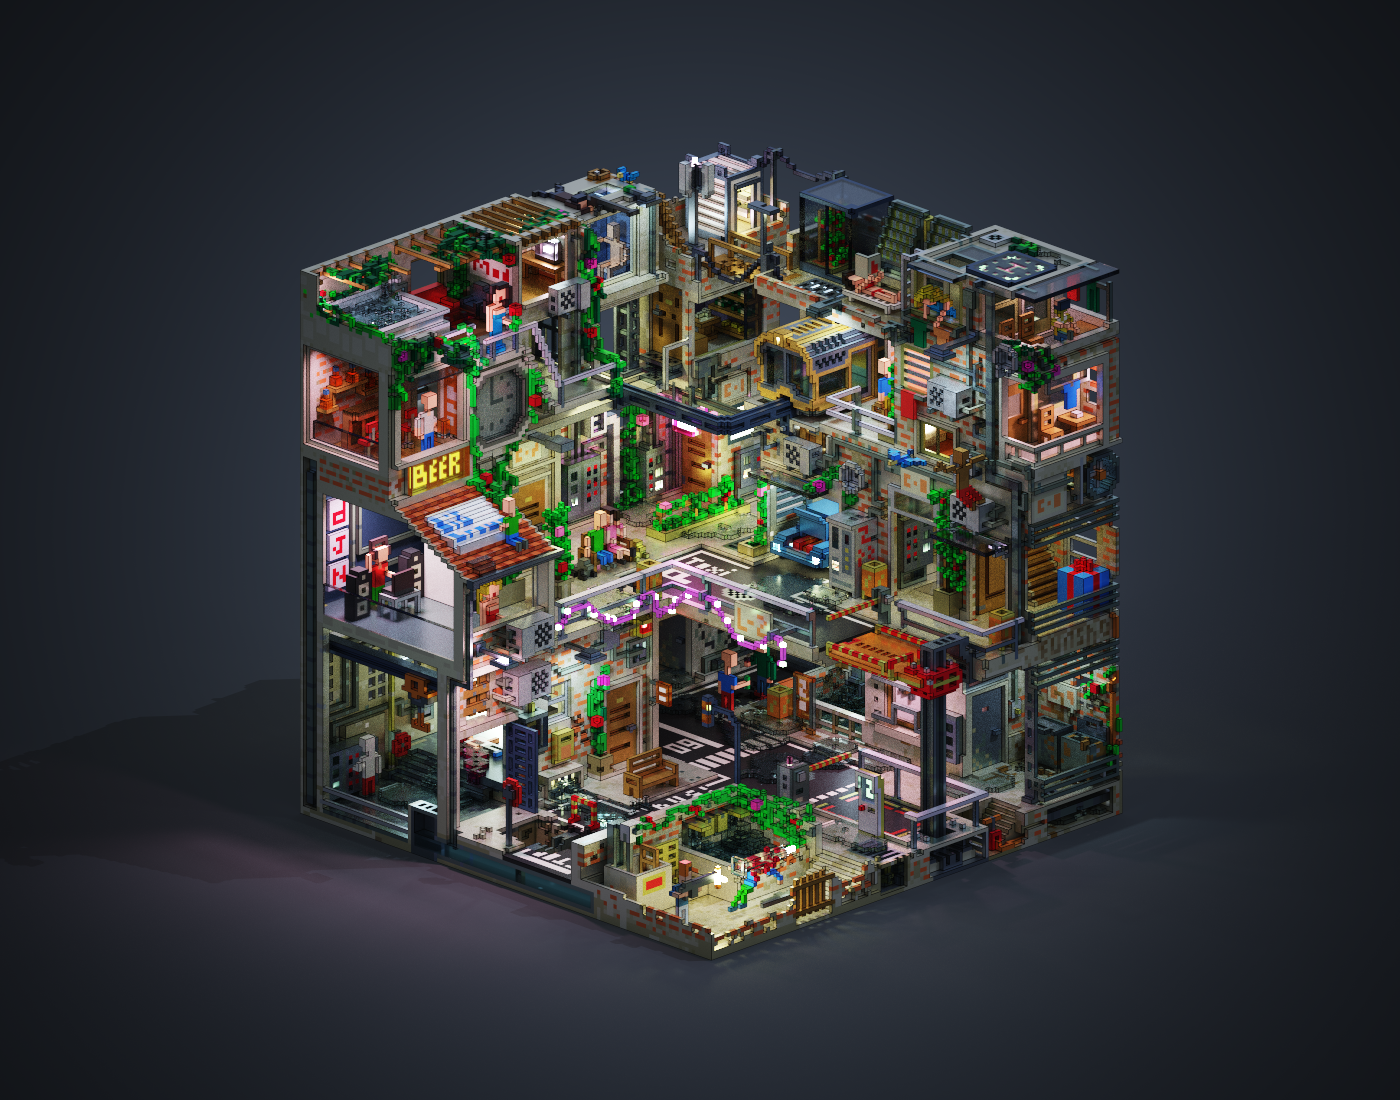
\includegraphics[width=.44\textwidth]{logos/voxel_textured_cube.png}
    \caption{Left: A cube textured with a texture made up of texels. Right: A cube textured with a texture made up of voxels. Images from \cite{Bej:OpenGLEx} and \cite{Ing:VoxPeop}}
  \end{center}
\end{figure}

Obviously, a 3-dimensional object made up of voxels requires much more memory space than the 2-dimensional projection of that object using equal-sided texels would. This is why the use of voxels at a reasonable resolution only became a realistic option for commodity hardware with the conception of Out-of-Core techniques. As rendering of voxels is very costly, some optimizations have to be made in order to make them a viable option. The probably most important thing to note is that not the whole texture volume looked at has to be in memory. For instance, voxels that are fully covered by opaque voxels in front of them are not visible anyway and can therefore be ignored while processing the frame.

As can be seen in figure 4.2, a huge advantage of using voxels is that they do not have to depend on base meshes in order to display 3-dimensional bodies. Displaying a comparable 3-dimensional scene using texel-based texturing would require quite a complex base mesh geometry, placing more load on the graphics card. However, one drawback of voxel-based respresentation is body deformation, which requires special handling and is easier done with a base mesh \cite{laine2011efficient}. Voxels also have the very simple advantage of being capable of modeling terrains with overhanging cliffs or caves which is impossible using height maps. Voxels can be rendered as points, for instance in 3-dimensional scanning where they form point clouds. With a sufficient number of samples making up one of those point clouds, voxels make it possible to generate virtual solid objects without requiring precomputed model made up of triangles. Another advantage of voxels is their regular structure. This facilitates the solution of aliasing problems that would be hard to handle using triangulated models \cite{Crassin:2009:GRS:1507149.1507152}. \cite{Gobbetti:2005:FVM:1073204.1073277} wrote about a fully adaptive technique for rendering very detailed scenes whose textures are made up of voxels and named it ``Far Voxels''.

\section{Voxel-based Octrees}

This section gives an overview of how the concepts of voxels and octrees can be combined to build a very advantageous representation structure for 3-dimensional scenes.

A voxel-based texture can potentially require large amounts of memory. Furthermore, especially for objects in the scene far away from the viewer the full resolution is not required. Octrees lend themselves as intuitive structures for adaptive level of detail control.

\begin{figure}[h]
  \begin{center}
    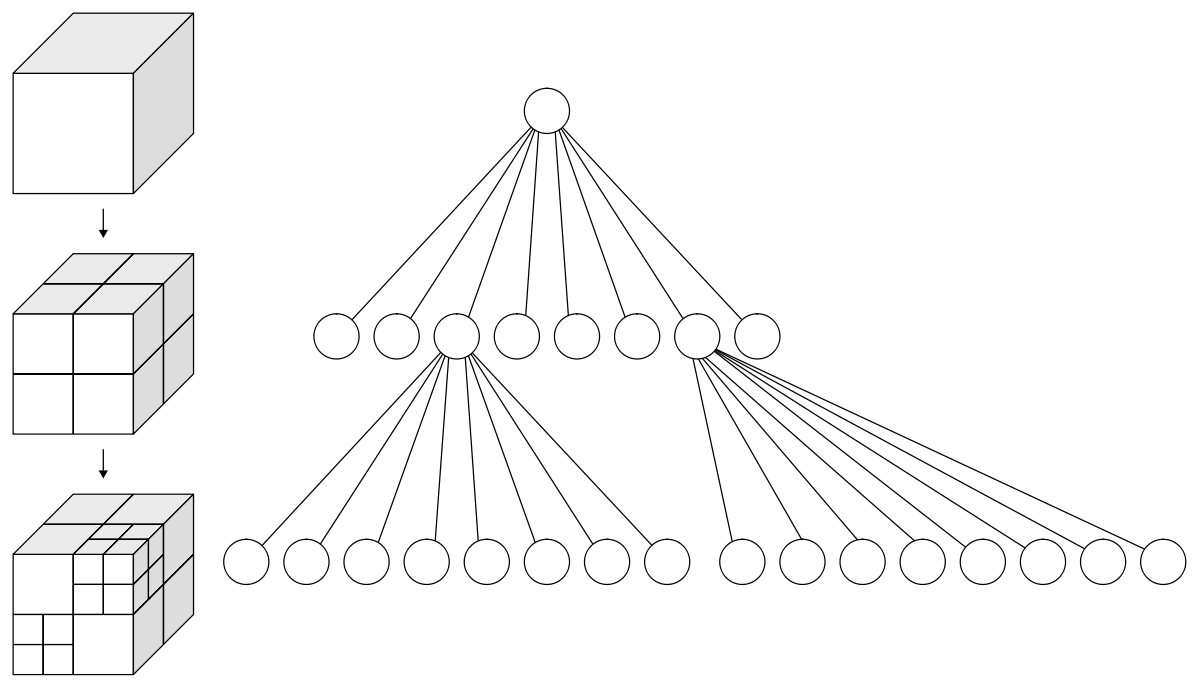
\includegraphics[width=.5\textwidth]{logos/voxel_octree_structure.png}
    \caption{Illustration of the structure of a voxel-based octree. Image from \cite{Wiki:Octree}}
  \end{center}
\end{figure}

As can be seen in figure 4.3, a node inside an octree can represent a 3-dimensional body - in this case a cube. In order to acquire the elements represented by the eight child nodes of this node, that body is sliced along the middle in all three dimensions, yielding eight cubes with half the parent cube's side length each. With this rule, a tree structure can be built by having a source 3-dimensional body and slicing it up to get as many depth levels as needed.

This concept can be transferred to voxel-based scene representation by taking a voxel as the smallest possible cube that can be represented by a node and taking the scene itself as the source body, following the procedure outlined above to generate an octree. However, the resulting octree does not provide any advantages yet as the information represented by it is redundant. The first levels contain very big data chunks and only the lower ones become more reasonable. This can be changed by, for example, setting a resolution limit for each node and downsampling represented data that exceeds this limit using filtering which works well with voxel-based textures. The octree resulting by following these steps contains a low-resolution version of the scene in its root node and resolution increases further and further as one descends along any path of the tree while the represented scene proportion decreases. 

\section{Example 1: GigaVoxels}

This section uses the discussed concepts to explain how GigaVoxels can be used to render large volumetric datasets with high performance. It will explain how this is related to both voxels and out of core processes.

\begin{figure}[h]
  \begin{center}
    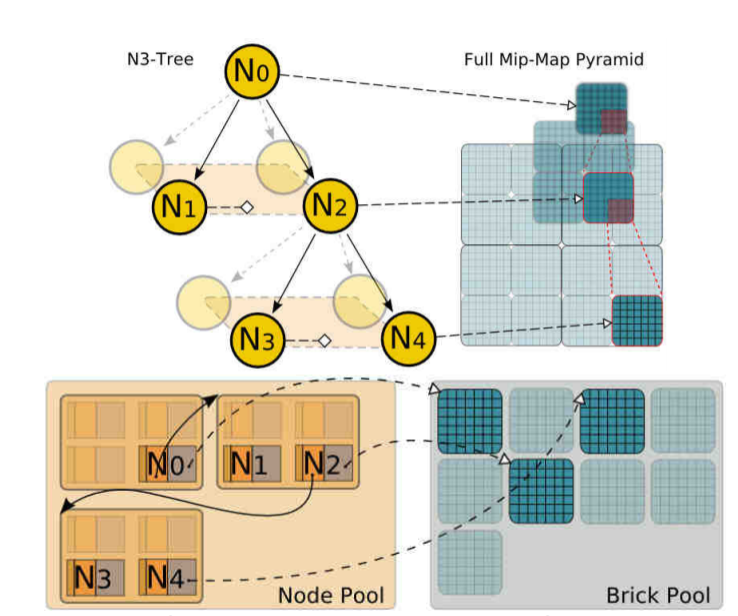
\includegraphics[width=.4\textwidth]{logos/gigavoxels_structure.png}
    \caption{Illustration of relation between the tree structure and brick detail. Image from \cite{Crassin:2009:GRS:1507149.1507152}}
  \end{center}
\end{figure}

\cite{Crassin:2009:GRS:1507149.1507152} came up with a structure that allows for interactive to real-time rendering of scenes with resolutions of 16384\textsuperscript{3} and higher. They also further increase detail by making use of procedural methods. One building unit of the algorithm they conceived are \textit{bricks}, which are small 3-dimensional grids of voxels approximating the part of the texture they represent. To get to the data needed for a specific part of the scene, they build and traverse an octree that stores pointers to such bricks inside its nodes or simply constants to indicate empty space. All loaded bricks of the scene are stored in the graphics card memory. However, this may exlude some bricks invisible due to being outside the view frustum or simply being covered - pointers to these bricks are invalidated. 

When the viewpoint changes, unavailable bricks are loaded on demand and level of detail of each loaded brick is adjusted as appropriate and needed in order to not oversubscribe memory. This adjustment is made exploiting the special structure of the octree: as the wanted mip-map level is searched, lower mip-map levels are passed in ascending order. This enables one to use them in calculations made to create a smooth transition between different tree configurations. If a missing brick is encountered during ray marching, the Z-buffer is used to block further execution along that ray until the required brick is loaded. In order to be able to continue execution from the last state, status information of the blocked ray is saved in a compressed format and communicated to the CPU.

By preferring higher mip-map levels over missing bricks of the same section, they finally introduce a moderate level of approximation to limit slow data transfer to an extent at which the promised interactiveness can be achieved.

\section{Example 2: ID Tech 5 Challenges}

This section discusses in detail how out of core rendering is compatible with parallelization using the ID Tech 5 Challenges example. It summarizes the faced challenges and how they were solved. 

\cite{van2009id} decided against using conventional virtual paging, because their textures with a side length of 1024 pages would have led to inacceptable performance due to thrashing. Instead, they went for the level of detail approach. With their solution, texture tiles becoming more detailed are upsampled first; further detail only starts being loaded after the higher-resolution tile has been acquired in the background.

As a frame of the scene would have required 38 milliseconds to be rendered at the required quality as opposed to a maximum available rendering time of 16 milliseconds in order to achieve 60 frames per second, parallelization became a necessity. Therefore, they developed a very invasive but highly scalable job processing system. Jobs are designed to never stall execution, be completely independent of other jobs and always complete - thus minimizing processing delays and bottlenecks.

The id Software team's approach shows that Out-of-Core techniques are indeed compatible with parallelization and therefore suited for future development as parallel programming becomes more and more crucial.

\chapter{Epilogue}
\label{ch:Epilogue}

As demonstrated, Out-of-Core techniques offer a very promising way of utilizing commodity graphics cards' potential in order to reach a renderable scene complexity far beyond what would be possible otherwise. 

A possible future step would be to elaborate on \cite{10.1007/978-3-540-40014-1_3}'s approach and exploit the next generations of graphics cards to create an even more realistic and immersive virtual reality experience. Also, further compression of output data representation and better prediction of occlusion and visibility events would be topics worth looking into \cite{Gobbetti:2005:FVM:1073204.1073277}.